\section{Dataset and Exploratory Data Analysis}
% [WRITING GUIDANCE]
% Target length: 1 column.
% Describe the source of the data and its original features.
% Discuss the target variable (Response) and its class imbalance.

% Insert Figure 1 here. (Dataset Overview / Missing Values)
\begin{figure}[htbp]
\centerline{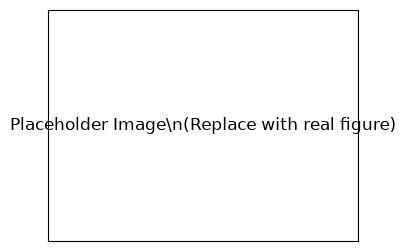
\includegraphics[width=\columnwidth]{figures/placeholder.png}}
\caption{Dataset Overview (Replace with actual missing values or descriptive plot).}
\label{fig:dataset_overview}
\end{figure}

% Insert Figure 2 here. (Target Distribution)
\begin{figure}[htbp]
\centerline{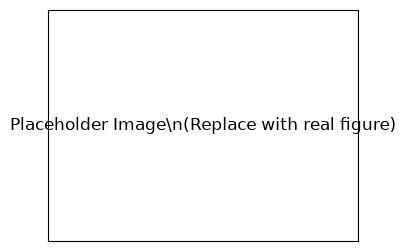
\includegraphics[width=0.7\columnwidth]{figures/placeholder.png}}
\caption{Target Distribution highlighting class imbalance.}
\label{fig:target_dist}
\end{figure}

% Insert Figure 3 here. (Correlation Matrix)
\begin{figure}[htbp]
\centerline{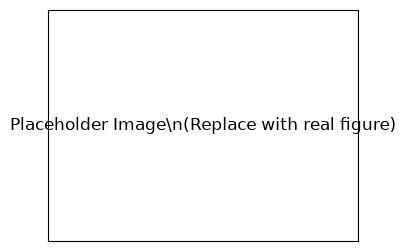
\includegraphics[width=\columnwidth]{figures/placeholder.png}}
\caption{Correlation Matrix of numeric features.}
\label{fig:correlation}
\end{figure}

% Insert Dataset Summary Table
\begin{table}[htbp]
\caption{Dataset Summary Statistics}
\begin{center}
\begin{tabular}{|l|c|c|}
\hline
\textbf{Feature} & \textbf{Data Type} & \textbf{Missing Values} \\
\hline
Income & Numeric & 24 \\
Education & Categorical & 0 \\
... & ... & ... \\
\hline
\end{tabular}
\label{tab:dataset_summary}
\end{center}
\end{table}

% Write your dataset description and EDA findings here...
